\documentclass[13pt, a4paper]{article}
\usepackage[utf8]{inputenc}
\usepackage{fontenc}
\usepackage{xcolor}
\usepackage{hyperref}
\usepackage[italian]{babel}
\usepackage[inline]{enumitem}
\usepackage{graphicx}
\usepackage{cleveref}

\setlist[enumerate,1]{label=\arabic*}
\setlist[enumerate,2]{label=\theenumi.\arabic*}
\setlist[enumerate,3]{label=\theenumii.\arabic*}

\graphicspath{ {res/} }
\usepackage{url}
\usepackage{acronym}
%\usepackage{natbib}
\usepackage{makeidx}
\usepackage{listings}
\usepackage[square,numbers,sort]{natbib}
\usepackage{tabularx}
\usepackage{float}

% version
\newcommand{\versionmajor}{0}
\newcommand{\versionminor}{1}
\newcommand{\versionpatch}{2}
\newcommand{\version}{\versionmajor.\versionminor.\versionpatch}
\newenvironment{inlinelist}{\begin{enumerate*}[label=\emph{(\roman*)}]}{\end{enumerate*}}
\typeout{Document version: \version}

% acronyms
\acrodef{FC}{Field Calculus}
\acrodef{AC}{Aggregate Computing}
\acrodef{dsl}[DSL]{Domain Specific Language}
\acrodef{ast}[AST]{Abstract Syntax Tree}
\acrodef{xc}[XC]{eXchange Calculus}
\newcommand{\ck}{\emph{Collektive}}

\title{\LARGE
    Un approccio unificante alla programmazione di dispositivi eterogenei nell'edge-cloud continuum \\ \small Prima relazione trimestrale di progetto
}

\author{
   Borsista: \\Angela Cortecchia \\ \small angela.cortecchia@unibo.it
    \and
    Tutor accademico: \\Danilo Pianini \\ \small danilo.pianini@unibo.it
}

%\date{\small Academic year}
%\makeindex

\begin{document}
\maketitle
\clearpage

%%%%%%%%%%%%%%%%%%%%body%%%%%%%%%%%%%%%%%%%%

\section{Recap del contesto}
\label{sec:context}
In un contesto in cui sono sempre in maggior numero i dispositivi dotati di capacità computazionali,
    che presentano la necessità di un'organizzazione e di un coordinamento tra loro,
    è necessario trovare una soluzione uniforme che permetta di programmare il comportamento e la coordinazione dei dispositivi.

Questi dispositivi possono essere di natura eterogenea, ovvero possono avere architetture e sistemi operativi diversi,
    e possono essere distribuiti in un'area geografica più o meno estesa.
%
La diversa natura di questi dispositivi può portare a problemi di interoperabilità e di comunicazione tra di essi.
%
Possono trovare applicazioni in vari contesti diversi, come ad esempio \emph{smart cities}, \emph{swarm robotics} e \emph{crowd management},
    includendo dispositivi di tipo wearable come smartwatch e smartphone.

La gestione del singolo dispositivo in questi contesti non è banale, possono ad esempio essere presenti 200 o più dispositivi
    connessi tra loro all'interno di una rete.
%
Gestirli tutti individualmente porterebbe a problemi di scalabilità, manutenibilità ed etereogeneità.

Per questi motivi si vuole passare dall'approccio classico con ``device centrico'', ovvero dove il programma è scritto per il singolo dispositivo,
    ad un approccio collettivo basato sulla programmazione macroscopica del comportamento dei dispositivi,
    usando tecniche di \emph{\ac{AC}}.

\ac{AC} è un paradigma di programmazione che permette di definire un unico comportamento di un insieme di dispositivi,
    definendo l'interazione fra loro.
%
È fondato sull'astrazione del \ac{FC} che consente di esprimere il comportamento auto-organizzante di reti
    di dispositivi come funzioni riutilizzabili che operano sui campi, dette ``costrutti'' o ``blocchi''.

Per fare ciò, viene sviluppato un \ac{dsl}, denominato \ck{}, basato sui concetti di \ac{AC} e \ac{FC} ed implementato in Kotlin Mulitplatform,
    che permette di scrivere codice in Kotlin e di compilarlo per diverse piattaforme, come JVM, JS, Native, iOS e Android.

\section{Obiettivi raggiunti}\label{sec:obiettivi-raggiunti}

Nella \Cref{fig:timeline} è mostrata la timeline indicativa del progetto, con i task da svolgere e la relativa durata.
%
Al momento ci troviamo tra M3 e M4, in corrispondenza della linea arancione.
%
Di seguito illustrerò i task svolti fino ad ora.

\begin{figure}
    \centering
    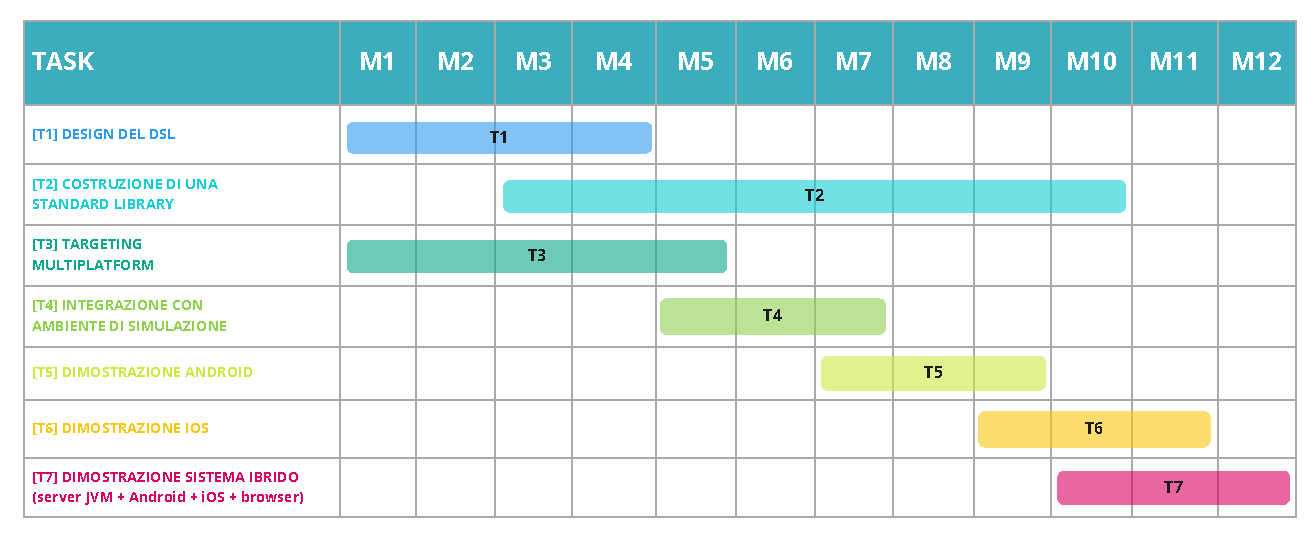
\includegraphics[width=\textwidth]{images/collektive_timeline}
    \caption{Timeline indicativa del progetto.}
    \label{fig:timeline}
\end{figure}

\subsection{Task T1 [Design del DSL]}\label{subsec:t1}

\paragraph{DSL}
Per prima cosa è servito capire quali fossero effettivamente i costrutti necessari da inserire all'interno del DSL di \ck{}\footnote{
    Repository con codice open source visitabile al seguente link \url{https://github.com/Collektive/collektive}.
}.
%
Tra i vari approcci proposti per l'implementazione del \ac{FC}, è stato scelto di utilizzare \ac{xc}.
%
\ac{xc} è un linguaggio di programmazione sperimentale per lo sviluppo di sistemi distribuiti omogenei che segue le astrazioni
    di \ac{AC}.

Astraendo da concorrenza, perdita di messaggi, protocollo di comunicazione di rete e fallimenti dei nodi,
    \ac{xc} permette di definire un modello di calcolo distribuito che si basa su un insieme di regole di trasformazione
    che operano sui campi computazionali,
    rivelandosi un modello di calcolo ideale per il progetto.

\ac{xc} è basato su una primitiva di comunicazione che permette di scambiare messaggi tra dispositivi --\emph{exchange}--,
    con l'aspetto cruciale che può inviare messaggi con valori diversi a seconda del vicino, consentendo un'interazione
    personalizzata tra essi.
%
Utilizzando questo costrutto è possibile implementare gli altri costrutti del \ac{FC}.

Identificato dunque il costrutto di base del \ac{dsl}, è stato possibile implementare altri costrutti per la comuncazione
    con peculiarità diverse, quali:
\begin{itemize}
    \item \emph{exchange}: per lo scambio di messaggi personalizzati tra dispositivi, restituendo al programma lo stesso
        valore che viene inviato ai vicini;
    \item \emph{exchanging}: come \emph{exchange}, ma restituisce un valore diverso da quello inviato;
    \item \emph{share}: implementato in termini di \emph{exchange}, permette di condividere un valore ai vicini, indistintamente
        dal destinatario, restituendo al programma il valore condiviso;
    \item \emph{sharing}: come \emph{share}, ma restituisce un valore diverso da quello condiviso;
    \item \emph{repeat}: costrutto del \ac{FC} che permette di modellare l'evoluzione nel tempo dello stato del dispositivo.
        In quanto non è necessaria comunicazione con i vicini, non è stato implementato in termini di \emph{exchange}.;
    \item \emph{repeating}: come \emph{repeat}, ma restituisce un valore diverso da quello restituito dall'iterazione precedente.
    \item \emph{neighboring}: costrutto del \ac{FC} che permette di accedere ai valori dei vicii e inviare loro informazioni,
        permettendo così di modellare l'evoluzione dell'informazione nello spazio.
        Implementato sia in termini di exchange che non, con differenze in termini di performance.
\end{itemize}

L'utilizzo di \ac{xc} porta un'innovazione aggiuntiva, in quanto al momento lo stato dell'arte non prevede l'implementazione di
    questa primitiva all'interno di un \ac{dsl}.


\paragraph{Compiler Plugin}

Per permettere una corretta comunicazione dei dispositivi, esiste il concetto di ``allineamento''.
%
La semantica del \ac{FC} è definita compositiva ed i messaggi scambiati tra vicini vengono automaticamente abbinati
    allo stesso costrutto del programma, determinato da un processo chiamato allineamento.
%
Ogni costrutto genera un ``export'', un valore di dati da inviare ai vicini, creando quindi un enriched \ac{ast} fino a quel costrutto.
%
Questi export vengono raccolti in un messaggio da trasmettere ai vicini, che può essere modellato come
    un albero ordinato di valori ottenuti durante la valutazione di ogni sottoespressione del programma.

Il meccanismo di allineamento assicura che ogni sotto-programma di un dispositivo sia abbinato al corrispondente dei vicini,
    seguendo un percorso identico nell'albero di valutazione,
    permettendo cosi di far comunicare i dispositivi allineati tra di loro.

Per fare ciò, è stato implementato un plugin per il compilatore di Kotlin, che si occupa di annotare le funzioni visitate
    durante la valutazione del programma, in modo da poter creare un path di esecuzione che permetta di allineare i dispositivi
    tra di loro.

\subsection{Task T2 [Costruzione di una standard library]}\label{subsec:task-t2-[costruzione-di-una-standard-library]}

\subsection{Task T3 [Targeting multiplatform]}\label{subsec:task-t3-[targeting-multiplatform]}

\section{Prossimi obiettivi}\label{sec:prossimi-obiettivi}

%completamento t1 t3
%implementazione standard library in contrapposizione a quella di protelis -francia
%ulteriori sviluppi di t4
%investigare integrazione con pulverization



%%%%%%%%%%%%%%%%%%%%end%%%%%%%%%%%%%%%%%%%%

% add more ....

\cite[none]{none}
\bibliographystyle{plain}
\bibliography{bibliography}

\end{document}